\chapter{Mettre en place un processus qui intègre l’ensemble des acteurs}
On parle ici d’un projet nécessitant recherche et développement technologique. Aussi, la recherche vient alimenter le développement, qui s’adapte aux besoins de la recherche. Plusieurs outils sont partagés par les différentes équipes : d’une part les outils développés par Teklia qui permettent l’extraction et la lecture \gls{HTR}, et d’autre part, des outils plus simples pour la gestion du projet.  

    \section{Une chaîne de traitement intégrée}

SocFace est un projet où la technologie joue un rôle clef. Il est donc nécessaire d’assurer un processus de traitement (workflow). La chaîne de traitement concerne la production de la base de données\footnote{Voir Annexe A}. 

\begin{figure}[H]
        \centering
        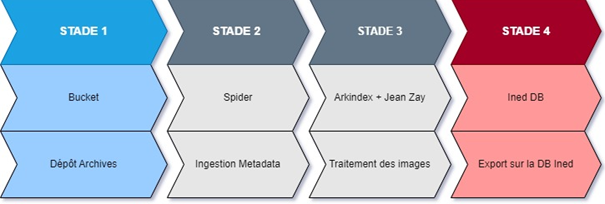
\includegraphics[width=1.0\linewidth]{Figures/Partie 1/Fig.1.3 - Extrait du panorama général des process.png}
        \caption[Extrait du panorama général des process]{Extrait du panorama général des process}
        \label{fig:Fig1.3}
    \end{figure}

Ce processus commence avec les services d’archives. Ils sont contactés par SocFace, qui leur propose de participer au projet. Comme on l’a dit, le taux de réponse est plutôt positif. Lorsque les services d'archives sont prêtes, elles donnent les listes de recensement sous forme d’images \gls{IIIF}\footnote{Voir Glossaire}, ainsi qu’un fichier qui contient les métadonnées associées aux images. Elles peuvent livrer un disque dur, ou bien se connecter sur les serveurs de Teklia. Il faut ajouter que parfois, les services d’archives utilisent une solution externe, comme Naoned. Plusieurs sont dans ce cas, c’est pourquoi les équipes du projet se sont rapprochées directement de ces fournisseurs de solutions pour regrouper les transferts de fichiers. Cette étape du processus peut prendre beaucoup de temps, soit parce que les images n’ont pas été encore numérisées, soit parce que des problèmes techniques ralentissent le transfert. De fait, tous les services d’archives n’ont pas les mêmes moyens humains, ni le même niveau d’expertise concernant ces questions. Ces échanges sont assurés par des équipes de l’INED ou parfois par Teklia, lorsque des questions plus précises sur les serveurs sont abordées. Si les services semblent hésiter, l’aide du SIAF est demandée. 

\begin{figure}[H]
        \centering
        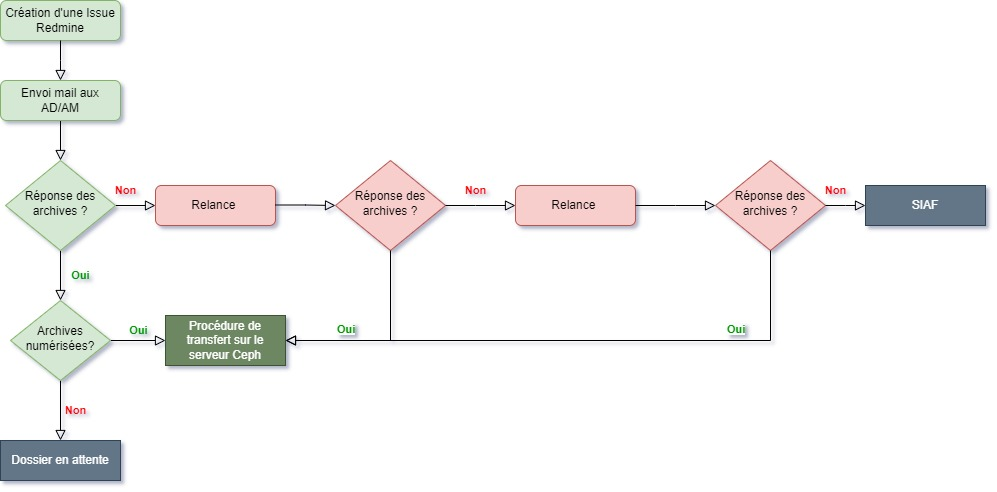
\includegraphics[width=0.8\linewidth]{Figures/Partie 1/Fig.1.4 - Contact Archives .jpg}
        \caption[Processus de contact des archives]{Processus de contact des archives}
        \label{fig:Fig1.4}
    \end{figure}

Une fois les données reçues, le travail sur l’image commence. Les images livrées par les services d’archives sont téléchargées dans l’outil \Spider{}. Une fois associées à leurs métadonnées, elles sont exportées ensuite sur l’outil \Arkindex{}, qui va opérer la magie de l’\gls{HTR} : reconnaissance et classification des pages, reconnaissance des \gls{entités} et regroupement en foyer (\textit{\gls{households}})\footnote{Voir Glossaire}, puis export de ces informations dans la base de données de l’INED. Ces différentes étapes sont assurées par les équipes de Teklia, qui possèdent la compétence informatique. Ces outils ont d’ailleurs été conçus par Teklia. Le process tel qu’il est décrit ici parait très simple, mais les spécificités techniques nécessitent en réalité de constants ajustements.

    \section{Les différents outils utilisés pour le projet}

Afin de bien comprendre l’ampleur de SocFace, il faut commencer par comprendre les outils utilisés par l’ensemble des équipes. Ces outils ont été développés pour la plupart par Teklia, qui en assure également la gestion quotidienne.

        \subsection{SPIDER}

Cet outil\footnote{Voir Annexe D} permet d’associer les images, généralement en .jpeg, avec un fichier de métadonnées également fourni par les archives, sous format .xml ou .csv (si le fichier est en .xml, il est nécessaire de le convertir en .csv via un script Python). Ces métadonnées identifient dans chacune des images : la commune et l’année. Parfois, il y a un chemin \gls{ARK}\footnote{Voir Glossaire}, ce qui permet de retrouver les images beaucoup plus facilement.  
L’outil \Spider{} est connecté aux serveurs contenant les images. Ces serveurs sont également gérés par Teklia. Il est souvent nécessaire de recommencer le traitement plusieurs fois, et même dans ce cas, on peut avoir des erreurs. Cela dépend beaucoup de la qualité du fichier de métadonnées fournit par les Archives. Ceux-ci sont en effet très hétérogènes. On aurait pu penser que fournir un modèle à suivre pour la fourniture des métadonnées aurait été plus utile pour le projet. Mais cela se serait révélé en réalité contre-productif : les services d’archives auraient pu remettre leur participation en question s’il avait fallu adapter leurs propres fichiers. 
Une fois les images associées entre elles, elles sont envoyées sur l’outil \Arkindex{}.

\begin{figure}[H]
        \centering
        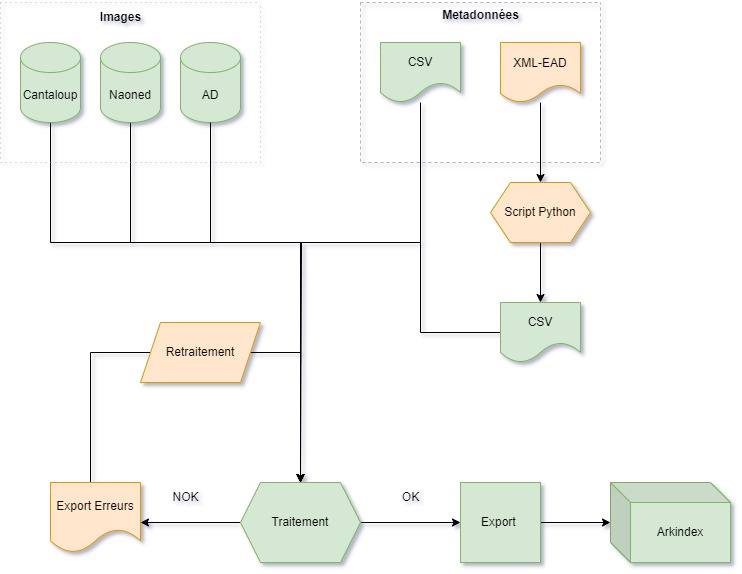
\includegraphics[width=0.8\linewidth]{Figures/Partie 1/Fig.1.5 - Processus Spider.jpg}
        \caption[Processus de l'outil \Spider{}]{Processus de l'outil \Spider{}}
        \label{fig:Fig1.5}
    \end{figure}

        \subsection{ARKINDEX}

\Arkindex{}\footnote{Voir Annexe C} est l'outil principal de Teklia qui permet de convertir les images numérisées en texte, de reconnaître les \gls{entités}\footnote{Voir Glossaire}, et d'exporter ces données vers une base de données.

\begin{figure}[H]
        \centering
        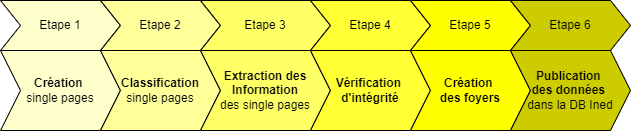
\includegraphics[width=0.8\linewidth]{Figures/Partie 1/Fig.1.6 - Arkindex General.png}
        \caption[Processus de l'outil \Arkindex{} (Général)]{Processus de l'outil \Arkindex{} (Général)}
        \label{fig:Fig1.6}
    \end{figure}

Avant de pouvoir lire et extraire les informations des images numérisées et les exporter dans la base de données, il faut travailler sur les pages. Les listes de recensement sont contenues dans de grands registres : il faut s’assurer que chaque page est traitée indépendamment de la page suivante, ce qui serait une double page. La technologie détecte donc naturellement une double page, mais l’outil va les découper pour créer des \gls{SP}\footnote{Voir Glossaire}, beaucoup plus facile à traiter. 
Une fois les pages découpées, elles sont classifiées : la machine identifie les premières pages, les dernières pages et les pages intermédiaires. Pour cela, elle est entraînée via des modèles : on lui donne des images déjà classifiées pour lui apprendre à reconnaître les types de pages et le modèle est ensuite appliqué aux images des archives via des workers¸c’est-à-dire des scripts qui tournent en arrière-plan. 
Le cœur de l'\gls{HTR} commence ensuite : en utilisant des modèles entrainés, les images sont analysées, et les informations extraites. Ces modèles n’ont pas été créés par Teklia, mais récupérés en Open Source. Les deux principaux sont \gls{DAN} et \gls{YOLO}. \YOLO{} a été créé par Joseph Redmon en 2016.  C’est un algorithme de détection d'objets en temps réel qui analyse une image en une seule passe pour identifier et localiser les objets. L’algorithme divise la page en plusieurs boites et effectue des prédictions en fonction de la façon dont il a été entraîné. Son avantage est qu’il travaille sur toutes les cases en même temps, là où les précédents modèles avaient besoin de repasser plusieurs fois sur la page. \DAN{}\footnote{Pour plus d'informations, cf le \href{https://github.com/FactoDeepLearning/DAN}{GitHub} du projet} a été créé par Denis Coqueret et est également orienté sur la reconnaissance manuscrite, et l’extraction d’information. 
Ces modèles doivent être entraînés pour fonctionner sur les images des archives. Il faut donc les nourrir avec des images déjà analysées et indexées. Pour cela, Teklia a créé Callico, qui permet de lancer des campagnes d’indexation. En faisant appel à des volontaires ou des étudiants rémunérés, des centaines de pages sont traitées correctement, avec détection manuelle des zones, et indexation du texte. Ces pages sont ensuite intégrées au modèle, qui peut dès lors prédire des pages non traitées en fonction des informations qu’il a apprises. C’est l’utilisation du \gls{DL} pour la reconnaissance manuscrite : on entraîne la machine à apprendre à détecter les informations pour qu'elle finisse par les reconnaître sans entraînement. Cela nécessite un nombre considérable de données d’entraînements : plus la machine apprend, plus elle devient experte. Ces outils sont très efficaces pour l'extraction des mentions simples comme les noms ou les dates, mais connaissent des difficultés avec les adresses. De fait, celles-ci sont souvent orientées verticalement, contrairement aux autres informations. Il faut donc apprendre aux modèles à orienter leur lecture différemment. 
Il faut noter que ces outils fonctionnent grâce au serveur JeanZay, le supercalculateur du CNRS\footnote{Voir Chapitre 6}.

        \subsection{Metabase}
Une fois les données identifiées et extraites, elles sont exportées vers une base de données, hébergée par l’\gls{INED}. A cause de l’ampleur du projet, cette base de données est difficilement accessible et exploitable sans un programme adapté, en l’espèce, R. Il est difficile de naviguer dans cette base de données sans connaissances préalable, c’est pourquoi il a fallu trouver une autre solution d'accès. Le choix s’est porté sur Metabase\footnote{https://www.metabase.com/}, qui est accessible en OpenSource.\\

On voit donc que ce projet nécessite des outils exigeants, qui demandent un travail constant et poussé, mais qui peuvent également réaliser un travail puissant et de qualité. Leur articulation est fragile, et le process dans son ensemble prend un certain temps. Au-delà des outils développés par les ingénieurs informatiques de Teklia, qui agissent sur la donnée elle-même, on doit également mentionner les outils de gestions du projet, qui aident à la collaboration entre les équipes.  

    \section{Les outils de gestion}

Comme on l'a vu précédemment les différents outils sont utilisés par plusieurs équipes : L’\gls{INED}, Teklia et parfois le \gls{SIAF}. Le processus de production est majoritairement opéré par les équipes de Teklia, mais tout se fait en concertation avec l’INED. De même, le SIAF intervient lorsque des difficultés ou des lenteurs interviennent avec les services d’archives. Or, toutes ces équipes ne sont pas géographiquement dans les mêmes lieux. Teklia possède des bureaux parisiens mais une partie de leurs collaborateurs sont en région. Et bien entendu, les autres institutions sont chacune dans leurs locaux. Il faut donc s’entourer – dès le début du projet - d’outils de gestion de projet qui permettent d’assurer une fluidité dans les échanges et une entraide entre les membres des différentes équipes.\\ 
On utilise généralement la méthode \gls{AGILE}\footnote{Voir Glossaire} pour améliorer les échanges dans les projets informatique. SocFace est un projet hybride, avec du développement, mais aussi de la recherche. Dès lors, on retrouve quelques notions propres à AGILE, comme le découpage du projet en phase avec des itérations régulières : on avance petit à petit, dans les différentes composantes du projet. 

            \subsection{REDMINE}

REDMINE est un outil de gestion de projets, qui permet de créer des \textit{"issues"}, c’est-à-dire des tâches, chacune assignées à des \textit{"projets"}. Cet outil est primordial, en raison de l’ampleur du projet. Comme on l’a vu, il y a plusieurs phases et chacune correspond à un "projet". Elles sont concomitantes : on n'attent pas qu’une phase soit terminée pour commencer la suivante :

\begin{itemize}[label=\textbullet] % Change les puces en points noirs
    \item La collecte auprès des archives départementales ou municipales 
    \item Les campagnes d’annotations des volontaires
    \item L’entraînement des modèles 
    \item La production 
    \item La création de la base de données 
    \item L'appariement (linking)
\end{itemize}

Sur chacun de ces \textit{"projets"}, les équipes créent des tâches qui peuvent être assignés à n’importe quel membre et visible de tous les autres, qui peuvent également ajouter des commentaires. Cela permet de garder un historique complet des problèmes éventuellement rencontrés et des solutions trouvées. 
A noter qu’il existe également des GitLab, alimentés à la fois par les équipes de l’INED et de Teklia, qui permet de documenter les process et les technologies utilisées ainsi qu'un wiki commun. Ce point est essentiel pour permettre à chaque membre du projet de travailler en autonomie.

        \subsection{Les réunions}

Afin de favoriser la collaboration entre toutes les équipes, des réunions hebdomadaires sont mises en place entre l’INED, Teklia et PSE. Cela permet de faire un point sur l'avancement du projet, sur les questions et les nouvelles tâches à venir. Il y a également des réunions régulières avec le SIAF. Bien entendu, chacune des équipes organise aussi ses propres réunions. Il faut également noter l’utilisation d'un logiciel de discussion, afin de favoriser le dialogue entre les équipes.\\ 
Tous ces outils sont bien entendu utilisés pour la majorité des projets - de recherche ou non, informatiques ou non. Mais ici, la singularité est qu’il s’agit d’institutions différentes, donc avec des contraintes différentes, du matériel différent, un personnel différent. Ces outils sont utiles pour fluidifier le travail mais aussi pour assurer un bon dialogue et une communion entre des équipes qui n’étaient pas destinées à travailler ensemble : chacune des équipes doit apprendre à travailler avec le matériel de l’autre, à utiliser le vocabulaire de l’autre. Cela nécessite une adaptation. Car si on parle ici de collaboration, comme dans un projet classique, il s’agit aussi d’interdisciplinarité. Un chercheur en sociologie doit donc pouvoir comprendre le langage d’un ingénieur informatique qui lui doit pouvoir comprendre les besoins d’un démographe. Le fait de garder une trace écrite, dans le logiciel Redmine, mais aussi les comptes-rendus des réunions, permet de faciliter ce dialogue entre des disciplines et donc des compétences difficiles. Cette mise en place est primordiale pour des projets de cette envergure, afin d’éviter les erreurs de communication, ou des malentendus. D’autant plus que la très grande majorité du personnel travaillant sur le projet est en télétravail, ce qui limite les possibilités de régler les problèmes rapidement. \\
Le travail d’équipe nécessite donc la mise en place d’outil de travails communs, d’autant plus que ces équipes sont dispersées sur plusieurs sites, et appartiennent à des structures différentes.\\ 

Le projet SocFace incarne donc un exemple ambitieux d’interdisciplinarité, entre la recherche académique et numérique. Cela illustre également la manière dont les associations entre le public et le privé peuvent dynamiser la recherche et l’innovation. À travers l’étude de cette coopération interdisciplinaire, nous avons observé que loin d’être en opposition, ces deux secteurs se complètent en apportant chacun leur expertise spécifique. Cette complémentarité s’est révélée essentielle dans le développement des outils technologiques qui sous-tendent SocFace, tout en répondant aux exigences rigoureuses du domaine de la recherche scientifique. Après avoir analysé les fondements de ce partenariat, il est désormais important d’examiner la manière dont les données, sont gérées et valorisées. Nous allons donc examiner les défis liés à la collecte, l’intégration et l’analyse des données publiques. Ces données, souvent fragmentées et hétérogènes, nécessitent des méthodes innovantes pour en extraire toute leur richesse. Nous explorerons comment SocFace parvient à transformer ces informations brutes en connaissances exploitables, tout en assurant leur protection et leur intégrité.